\documentclass[11pt]{article}

\usepackage{amssymb,amsmath}
\usepackage{times,psfrag,epsf,epsfig,graphics,graphicx,caption}
\usepackage{enumitem}
\usepackage{algorithm}
\usepackage{algorithmic}

\begin{document}
\date{}

\title{PHSX 343: Assignment 6}

\author{William Jardee}

\maketitle


\section*{Problem 1}
    To get the middle two $y=y'$ and $z=z'$, we can just use the law of symmetry to show $y'=y$ and $z=z'$.\\
    Now to modify $x=\gamma (x'-vt')$ and $t = \gamma (t'+\frac{v}{c}x')$:
    \begin{center}
        $x' = \Big(\frac{1}{\gamma}\Big)x +vt'$ \quad $t' = \frac{t}{\gamma} - \frac{vx'}{c^2}$
    \end{center}
    \[x' = \Big(\frac{1}{\gamma}\Big)x + v\Big(\frac{t}{\gamma}-\frac{vx'}{c^2}\Big) = \frac{1}{\gamma}x +\frac{vt}{\gamma} - \Big(\frac{v}{c}\Big)^2 x\]
    \[\Big(1+\Big(\frac{v}{c}\Big)^2\Big)x' = \frac{1}{\gamma}x +\frac{vt}{\gamma}\]
    \[x' = \gamma x +vt\gamma = \gamma(x+vt)\]\\
    
    \begin{center}
        $x' = \Big(\frac{1}{\gamma}\Big)x +vt'$ \quad $t' = \frac{t}{\gamma} - \frac{vx'}{c^2}$
    \end{center}
    \[\frac{1}{\gamma} t = t' +\frac{v}{c^2}\Big(\frac{1}{\gamma}x +vt'\Big)\]
    \[\frac{1}{\gamma}t -\frac{v}{c\gamma}x = t'\Big(1 +\Big(\frac{v}{c}\Big)^2\Big) = \frac{1}{\gamma}t - \frac{v}{c^2 \gamma}x\]
    \[t' = \gamma t -\frac{v}{c^2}\gamma x = \gamma \Big( t - \frac{v}{c^2}x\Big)\]
    
    The trick of switching primes and chaning the positive to negative on the velocity works because that's exactly how you solve the problem when you flip the frames. The frames are now moving the opposite direction, but everything else has to be the same since the law of physics are the same for both frames. 

\section*{Problem 2}

\begin{enumerate}[label=\alph*)]
    \item 
        \parbox{0}{ 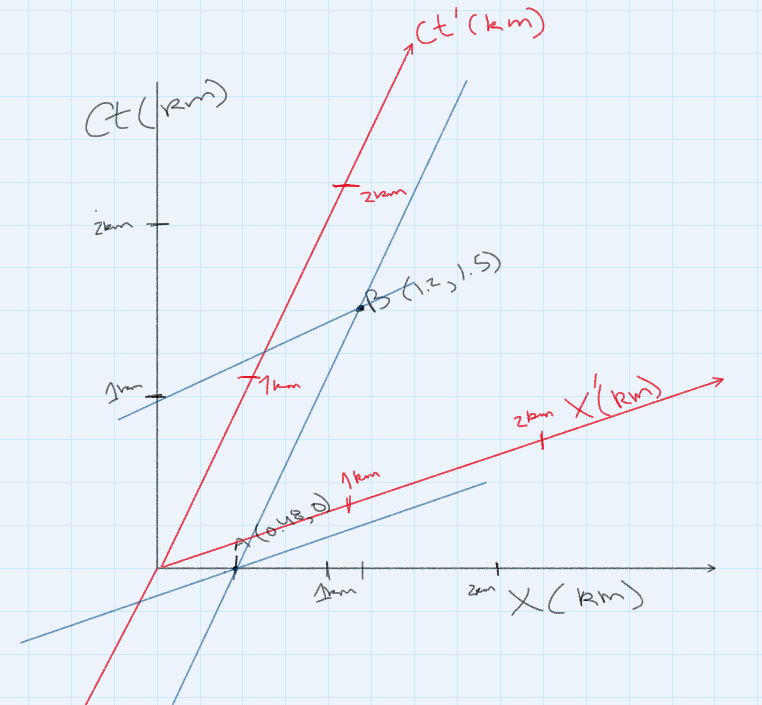
\includegraphics[width = 200pt]{Homework06/Homework1.PNG}}

    \item
        If we use the slope of the line given by connecting A an B, then we get the slope of $ct'$, or $\frac{\Delta t}{\Delta x} = \frac{720 m}{5 \times 10^{-6}} = 2.08 c \frac{s}{m}$. Of course the slope is $\frac{c}{v}$, so the speed of the frame is $v = 0.48$. Using this value in $\gamma$, the ratio of the axis is 1.399. You can see that the scaling on the axis is drawn in, this was a rough estimate from $\gamma$, so any values we read will be estimates. With that being said, $t'_a = -0.67 \mu s$ and $t'_b = 3.93 \mu s$. These are just approximations however, so $\Delta t' \approx 3.94 \mu s$\\
        Checking these numbers against the Lorentz transformation:
        \[t' = \gamma \Big(t-\frac{vx}{c^2}\Big)=4.39 \mu s\]
        While this is a decent amount off of what I said, the direction of change is the correct direction. I would attribute my error to improperly drawing the diagram. 
    \item
    Proper time happens when there is no change in location between the two events. The S' frame has the same $x$ location for both events, so it measures proper time
        
\end{enumerate}

\section*{Problem 3}

\begin{enumerate}[label=\alph*)]
    \item 
        \parbox{0}{ 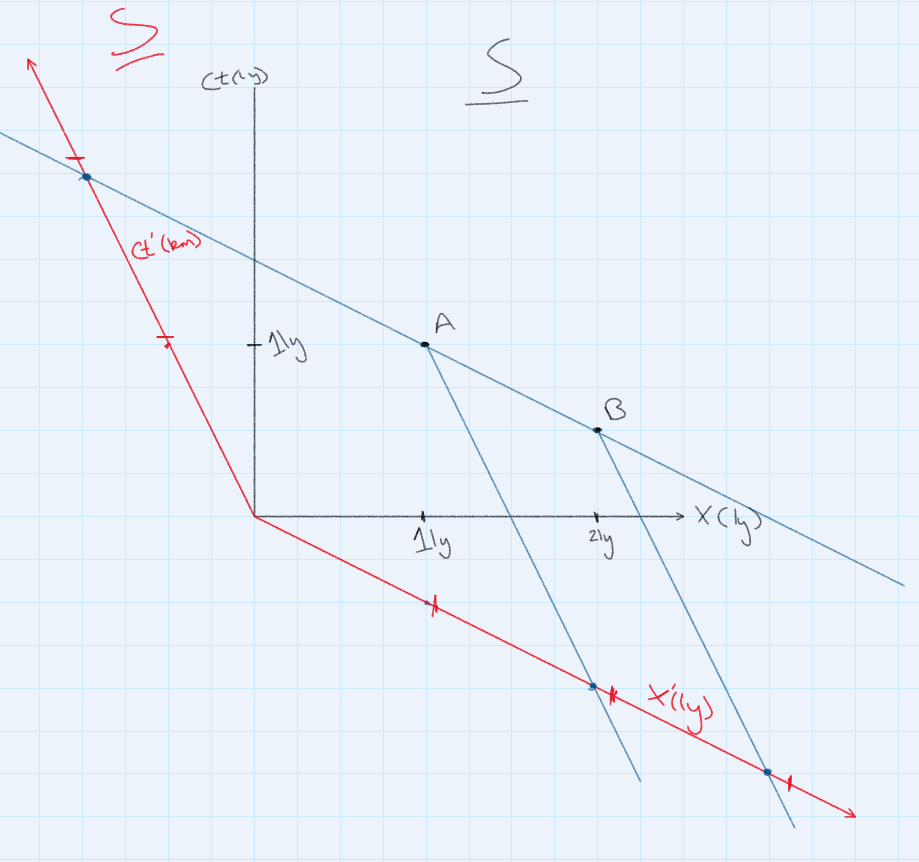
\includegraphics[width = 200pt]{Homework06/Homework2.PNG}}
        
    \item
        Like in problem 2, the answer that I get for the change in location are merely guesses from the graph. The accuracy of them depends on how well the plot was draw, and by it being draw by hand the error is exaggerated.\\
        I found the lines this time by taking advantage of the nice numbers provided. The slope created by connecting the points turned out to be $\frac{1}{4}$, since this is the slope for the x-axis, our speed becomes $v = 0.25c$. This gives us a $\gamma = 1.033$ and the resulting tick marks. Eye-balling the intersection, it seems that $x'_A = 1.9 km$ and $x'_B = 2.85$. This would make $\Delta x' = 0.95km$.\\
        Checking this against a Lorentz transform: 
        \[x = \gamma ( x' - vt') = \gamma x' \rightarrow x'=\frac{x}{\gamma} = 0.968 ly\]
        Comparing this to our estimate, they are rather close but there is still a margin of error, as to be expected.
    
    \item 
        Proper time is measured when you are at rest with the object. Measurement is taken with no passage of time, meaning that it is at rest while doing the measurement. So it would seem that S' gives the proper length of the object. 
        
\end{enumerate}


\end{document}
